\documentclass[xetex,mathserif,serif]{beamer}
\usepackage{polyglossia}
\setdefaultlanguage[babelshorthands=true]{russian}
\usepackage{minted}
\usepackage{tabu}

\useoutertheme{infolines}

\usepackage{fontspec}
\setmainfont{FreeSans}
\newfontfamily{\russianfonttt}{FreeSans}

\tabulinesep=0.7mm

\title{gRPC}
\author[Юрий Литвинов]{Юрий Литвинов \newline \textcolor{gray}{\small\texttt{yurii.litvinov@gmail.com}}}

\date{17.05.2017г}

\begin{document}
	
	\frame{\titlepage}

	\section{protobuf}

	\begin{frame}
		\frametitle{Protocol buffers}
		\framesubtitle{protobuf}
		\begin{itemize}
			\item Механизм сериализации-десерилизации данных
			\item Компактное бинарное представление
			\item Декларативное описание формата данных, генерация кода для языка программирования
			\begin{itemize}
				\item Поддерживается Java, Python, Objective-C, C++, Go, JavaNano, Ruby, C\#
			\end{itemize}
			\item Бывает v2 и v3, с некоторыми синтаксическими отличиями
			\item Хитрый протокол передачи, \url{https://developers.google.com/protocol-buffers/docs/encoding}
			\begin{itemize}
				\item До 10 раз компактнее XML 
			\end{itemize}
		\end{itemize}
	\end{frame}

	\begin{frame}[fragile]
		\frametitle{Пример}
		Файл .proto:
		\begin{minted}{protobuf}
message Person {
  required string name = 1;
  required int32 id = 2;
  optional string email = 3;
}
		\end{minted}
		Файл .java:
\begin{minted}{java}
Person john = Person.newBuilder()
    .setId(1234)
    .setName("John Doe")
    .setEmail("jdoe@example.com")
    .build();
output = new FileOutputStream(args[0]);
john.writeTo(output);
\end{minted}
\end{frame}

	\begin{frame}
		\frametitle{Технические подробности}
		Для Java:
		\begin{itemize}
			\item .proto-файлы --- в папку src/main/proto
			\item gradle-плагин com.google.protobuf
			\item \url{https://github.com/google/protobuf-gradle-plugin/blob/master/exampleProject/build.gradle}
		\end{itemize}
		Для остального: скачать и поставить protoc
		\begin{itemize}
			\item \url{https://github.com/google/protobuf}
		\end{itemize}
	\end{frame}

	\section{gRPC}

	\begin{frame}
		\frametitle{gRPC}
		\begin{columns}
			\begin{column}{0.6\textwidth}
				\begin{itemize}
					\item средство для удалённого вызова (RPC)
					\item Работает поверх protobuf
					\item Разрабатывается Google
					\item Поддерживает C++, Java, Objective-C, Python, Ruby, Go, C\#, Node.js
				\end{itemize}
			\end{column}
			\begin{column}{0.4\textwidth}
				\begin{center}
					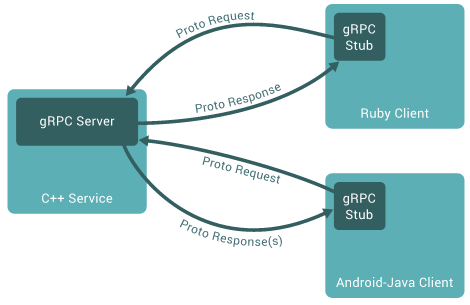
\includegraphics[width=\textwidth]{grpc.png}
				\end{center}
			\end{column}
		\end{columns}
	\end{frame}

	\begin{frame}[fragile]
		\frametitle{Технические подробности}
		\begin{itemize}
			\item Сервисы описыватются в том же .proto-файле, что и протокол protobuf-а
			\item В качестве типов параметров и результатов --- message-и protobuf-а
		\end{itemize}
		\begin{minted}{protobuf}
service RouteGuide {
  rpc GetFeature(Point) returns (Feature) {}
  rpc ListFeatures(Rectangle) returns (stream Feature) {}
  rpc RecordRoute(stream Point) returns (RouteSummary) {}
  rpc RouteChat(stream RouteNote) returns (stream RouteNote) {}
}
		\end{minted}
		\begin{itemize}
			\item Сборка --- плагином grpc к protoc
		\end{itemize}
\end{frame}

	\begin{frame}[fragile]
		\frametitle{Реализация сервиса на Java}
		\begin{scriptsize}
			\begin{minted}{java}
private static class RouteGuideService extends RouteGuideGrpc.RouteGuideImplBase {
    ...
    @Override
    public void getFeature(Point request, StreamObserver<Feature> responseObserver) {
      responseObserver.onNext(checkFeature(request));
      responseObserver.onCompleted();
    }

    @Override
    public void listFeatures(Rectangle request, StreamObserver<Feature> responseObserver) {
      for (Feature feature : features) {
        ...
        int lat = feature.getLocation().getLatitude();
        int lon = feature.getLocation().getLongitude();
        if (lon >= left && lon <= right && lat >= bottom && lat <= top) {
          responseObserver.onNext(feature);
        }
      }
      responseObserver.onCompleted();
    }
			\end{minted}
		\end{scriptsize}
\end{frame}

	\begin{frame}[fragile]
		\frametitle{Реализация сервиса на Java (2)}
		\begin{scriptsize}
			\begin{minted}{java}
    @Override
    public StreamObserver<RouteNote> routeChat(
            final StreamObserver<RouteNote> responseObserver) {
      return new StreamObserver<RouteNote>() {
        @Override
        public void onNext(RouteNote note) {
          List<RouteNote> notes = getOrCreateNotes(note.getLocation());
          for (RouteNote prevNote : notes.toArray(new RouteNote[0])) {
            responseObserver.onNext(prevNote);
          }
          notes.add(note);
        }
        @Override
        public void onError(Throwable t) {
          logger.log(Level.WARNING, "routeChat cancelled");
        }
        @Override
        public void onCompleted() {
          responseObserver.onCompleted();
        }
      };
    }
			\end{minted}
		\end{scriptsize}
\end{frame}

	\section{Задача}

	\begin{frame}
		\frametitle{Задание на пару}
		Разработать сетевой чат (наподобие Jabber) с помощью gRPC
		\begin{itemize}
			\item peer-to-peer, то есть соединение напрямую
			\item Консольный пользовательский интерфейс
			\begin{itemize}
				\item Отображение имени отправителя, даты и текста сообщения
			\end{itemize}
			\item Адрес peer-а и порт --- параметры
			\item Указание своего имени --- параметром или в конфигурационном файле
			\item Логирование
		\end{itemize}
	\end{frame}

\end{document}